\subsection{RQ2: batching costs at equal span retention}\label{sec:batch-results}
Bypass and retain-all tail export every span in each fixed-input cell. At 250 offered spans/s with JSON plus Jaeger, retain-all tail reduces Collector CPU relative to bypass at the 100\,ms batch timeout and increases it at 1,000\,ms. The respective mean differences are $-0.173$ and $+0.066$ CPU-seconds over sixty seconds plus five seconds of drain. Both directions occur in all eight paired blocks. Bypass consumes 0.249--0.603 CPU-seconds across the original configurations, below 1\% of one core.

\begin{figure}[htbp]
\centering
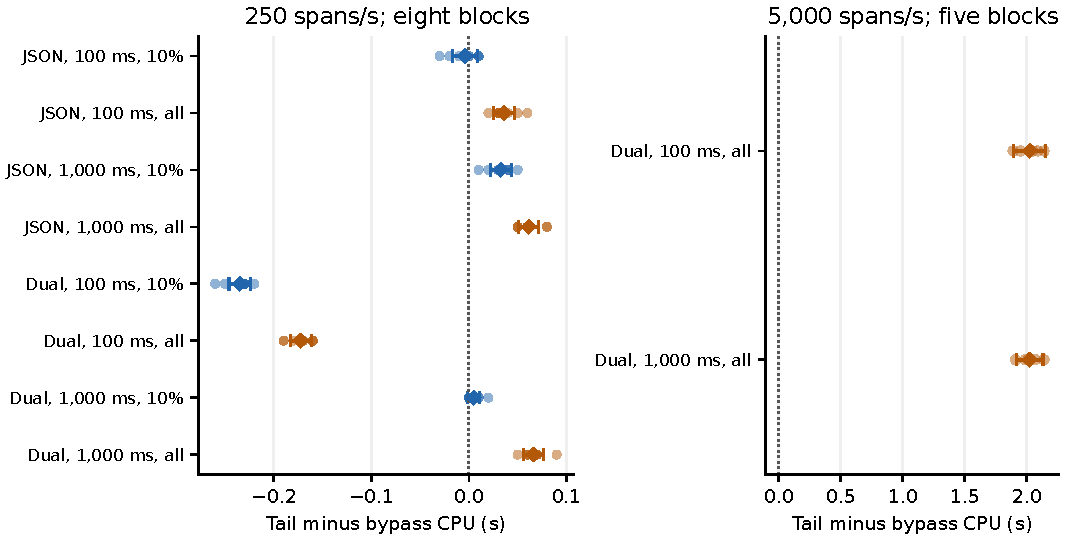
\includegraphics[width=\linewidth]{figures/controlled-cost-contrasts.pdf}
\caption{Fixed-input Collector CPU contrasts with bypass. Dots are paired runtime-block differences; diamonds and bars show means and pointwise 95\% Student-$t$ intervals. The original 250-span/s study has eight blocks; the separate 5,000-span/s study has five. Both measure sixty seconds of load plus five seconds of drain. The panels use different horizontal scales. Negative values mean less CPU than bypass. ``Dual'' means JSON plus Jaeger; ``all'' denotes retain-all tail.}
\label{fig:controlled-cost}
\end{figure}

At the lower rate, bypass sends 300 batches of fifty spans with the short timeout and sixty batches of 250 with the long timeout. Retain-all tail sends approximately sixty batches with either setting. The pinned processor's one-second policy ticker and per-trace forwarding explain how stateful release changes grouping~\cite{otelTailProcessor0136}. Adding Jaeger changes the retain-all tail-minus-bypass contrast by $-0.209$\,s at the short timeout but only $+0.005$\,s at the long timeout.

The reversal does not persist at the new 5,000-span/s operating point. Retain-all tail increases Collector CPU at both timeouts in every paired block. Mean differences are \HighBatchShortDifference{}\,s at 100\,ms, with interval \HighBatchShortInterval{}, and \HighBatchLongDifference{}\,s at 1,000\,ms, with interval \HighBatchLongInterval{}. Bypass now consumes about 4.9 CPU-seconds, or 7.6\% of one core over the measured window. Its 1,000 batches are all size-triggered at both timeouts. Tail emits 1,200 and 1,154 batches at the short and long timeouts respectively. It therefore no longer reduces batch count relative to bypass. Figure~\ref{fig:controlled-cost} reports both higher-rate contrasts alongside the original ones.

The batch target is a trigger rather than an exact output size~\cite{otelBatchProcessor0136}. Bypass adds fifty spans per request and crosses the 256-span target at 300; tail forwards five-span traces individually and crosses it at 260. At 100\,ms, residuals flush between policy releases: each measured cell records 1,139 size-triggered 260-span batches and 61 partial timeout batches. At 1,000\,ms, residuals accumulate across releases, giving 1,153 batches of 260 spans and one final timeout batch of 220, or $\lceil300{,}000/260\rceil=1{,}154$. These counts reconstruct all 300,000 measured spans in every block.

Serialization changes at equal span retention too. In the original measured corpus, bypass emits 600 resource/scope groups while retain-all tail emits 6,000, increasing JSON from about 4.99 to 7.05 million bytes. The file exporter serializes the grouping it receives~\cite{otelFile0136}. Reducing batch count can therefore coexist with increased serialized volume. Trace count, grouping, bytes, and CPU describe different properties of the pipeline.
